\documentclass{beamer}

\title{6 Degrees of Wikipedia}
\author{Troy Astorino, Neil Forrester}
\date{April 10, 2013}
\institute[6.834 -- MIT]{Cognitive Robotics \\ Massachusetts Institute of Technology}

\usepackage{graphicx}
\usepackage{amsmath}

\usetheme{CambridgeUS}
\usecolortheme{beaver}
\setbeamertemplate{section in toc}[square]
%\setbeamercolor{section number projected}[bg=black, fg=red]
\setbeamertemplate{navigation symbols}{} % remove navigation symbols

\begin{document}
\begin{frame}
  \maketitle
\end{frame}

\begin{frame}
  \frametitle{The 6 degrees of Wikipedia Game}

\begin{columns}
\begin{column}{0.45\textwidth}
  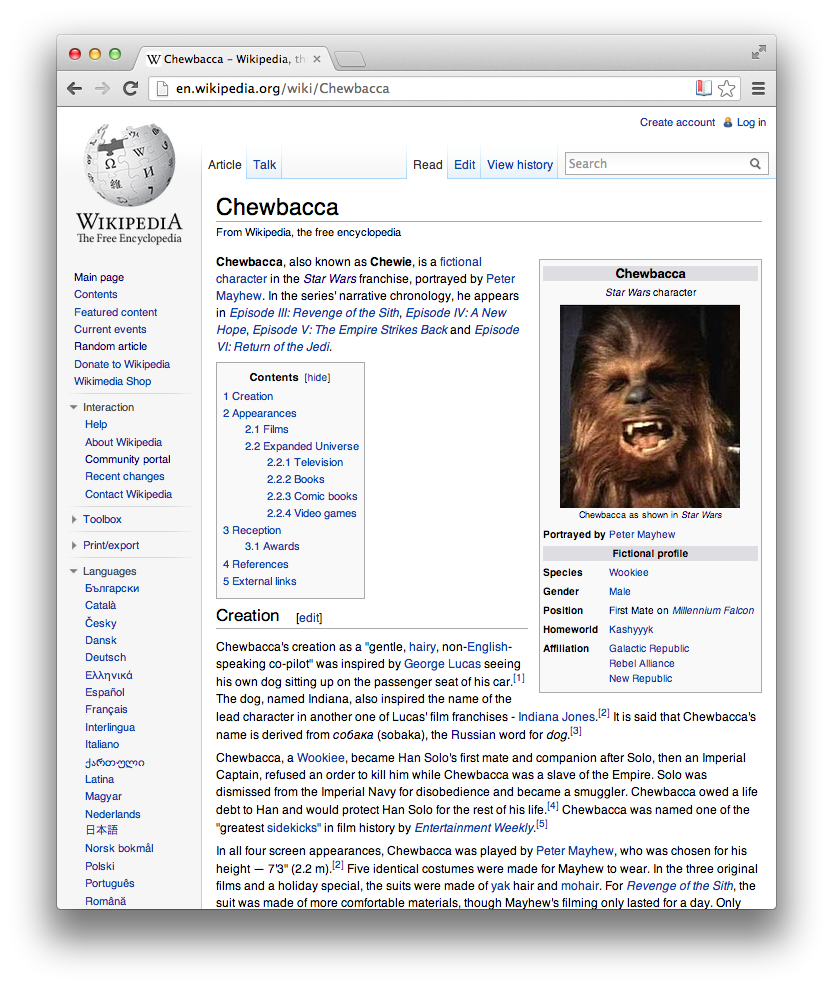
\includegraphics[width=2.25in]{img/chewbacca.png}
\end{column}

\begin{column}{0.1\textwidth}
$$ \Longrightarrow $$
\end{column}

\begin{column}{0.45\textwidth}
  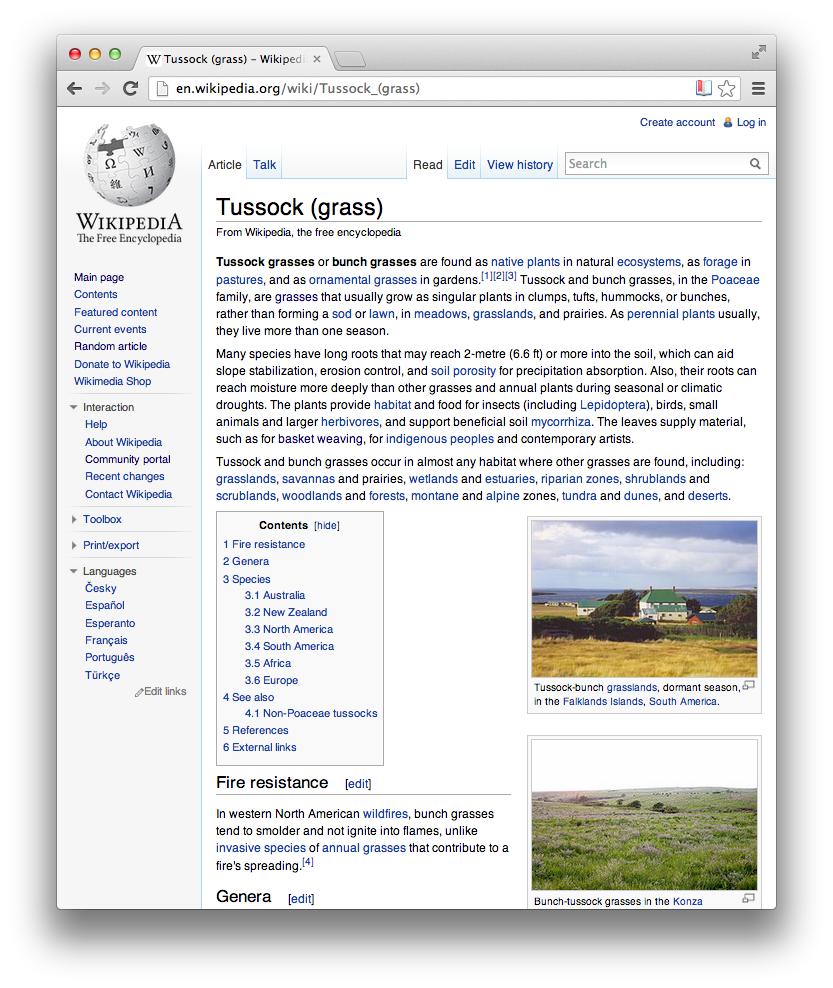
\includegraphics[width=2.25in]{img/tussock.png}
\end{column}

\end{columns}

\end{frame}

\begin{frame}
  \frametitle{Connection to co-occurences}

\begin{itemize}
  \item To fairly compete against a human, must fetch webpages \\
    \hspace{0.3in}$\longrightarrow$ expensive action

  \item Co-occurence model useful when have a search action is costly
\end{itemize}

\end{frame}

\begin{frame}
  \frametitle{Category Graph as Knowledge Graph}
\begin{itemize}
  \item Wikipedia articles divided into categories, gives knowledge of Wikipedia
    structure
  \item For an algorithm, a category graph can be the analog to a human's
    knowledge
    
  \item Use structure of category graph to inform search, as humans use
    relations between concepts

\end{itemize}
\end{frame}

\begin{frame}
  \frametitle{Probability that an article is in a category}

\[P(t_i \in c_j | t_i = [w_1, w_2, \dots, w_n]) = \frac{P(t_i = [w_1, w_2,
  \dots, w_n] | t_i \in c_j) P(t_i \in c_j)}{P(t_i = [w_1, w_2, \dots, w_n])}\]

\end{frame}

\begin{frame}
\frametitle{Assume independence of words}

\begin{multline*}
P(t_i = [w_1, w_2, \dots, w_n] | t_i \in c_j) \\
\begin{aligned}
& = P(w_1 \in t_i \cap w_2 \in t_i \cap \dots \cap w_n \in t_i | t_i \in c_j) \\
& \approx P(w_1 \in t_i | t_i \in c_j) P(w_2 \in t_i | t_i \in c_j) \cdots P(w_n
\in t_i | t_i \in c_j) \\
\end{aligned}
\end{multline*}

\end{frame}

\begin{frame}
\frametitle{Training data}

\[P(w_l \in t | t \in c_j) \propto \displaystyle \sum_{t \in c_j} \sum_l 
    \delta (w_l \in t)\]
such that
\[\displaystyle \sum_l P(w_l \in t | t \in c_j) = 1\]

\vspace{2em}

\[P(t_i \in c_j) = \frac{\text{\# of articles in } c_j}{\text{\# of articles}}\]

\end{frame}


\begin{frame}
\frametitle{Search strategy}

% The basic heuristic the algorithm uses to inform search is the shortest paths on
% the category graph between the current article and the goal article. This should
% naturally send the algorithm moving towards more general categories when it is
% farther from the goal article, and towards more specific articles when it is
% closer to the goal article. This is a good general strategy similar to what a
% human does, so this tendency is reinforced by explicitly encoding a weighting to
% move in this fashion. A centrality measure is used as an analog for the
% generality of a category, likely the eigenvector centrality or PageRank
% centrality, depending on whether the category graph is analyzed as a directed
% graph or an undirected graph. Thus, the algorithm incorporates the shortest path
% between the initial and goal articles and information on category generality in
% order to choose the target categories for the next link.  The algorithm then
% chooses the target categories based on the calculated probability of the
% articles being in those categories.

\end{frame}

\begin{frame}
\frametitle{Limiting scope of Wikipedia}

\begin{itemize}
\item Consider only the $x$ most viewed articles. Only include categories that
  these articles are in.

\item Consider only the top $x$ categories ranked by number of pages in the
  category. Only include pages in those categories.

\item Consider only the top $x$ categories ranked by number of subcategories in the
  category. Only include pages in those categories.

\item Consider only articles with more than $x$ words. Only include categories
  those pages are in.
\end{itemize}

\end{frame}

\begin{frame}
  \frametitle{Current Status}
  \begin{itemize}
  \item Loading database of Wikipedia pages, categories, and links has been much
    more difficult and taken much longer than expected (thank you Eric for
    helping us out!)
    \item Thoroughly thinking script to ensure that don't make a costly mistake
  \end{itemize}

\end{frame}
\end{document}